%Fiquemos com Deus e Nossa Senhora!
%Sao Jose de Cupertino rogai por nos!!
%Honra teu pai e tua mae!
% ### Uses XeLaTeX ### %
% ### Needs beamer-master ### %
\documentclass[aspectratio=169]{beamer} %. Aspect Ratio 16:9

\usetheme{AI2} % beamerthemeSprace.sty
\usepackage[portuguese]{babel}
\usepackage[utf8]{inputenc}
\usepackage[T1]{fontenc}
\usepackage{ragged2e,bm,oubraces,tikz}
\usepackage{algorithmic}
\DeclareMathOperator*{\argmin}{arg\,min}
\DeclareMathOperator*{\argmax}{arg\,max}

\newcommand*\mycirc[1]{%
  \begin{tikzpicture}
    \node[draw,circle,inner sep=2pt] {#1};
  \end{tikzpicture}}
  
 \newenvironment{algorithm}{\begin{quote} %\vspace{1em}
\begin{algorithmic}\samepage}{\end{algorithmic} %\vspace{1em} 
\end{quote}}

% DATA FOR FOOTER
\date{2025}
\title{- Teoria da Computação e Linguagens Formais}
\author{João Paulo Papa}

\begin{document}
% ####################################
% FIRST SLIDE 						:: \SliTit{This is the Title of the Talk}{A. B. Name}{Sprace}
% SUB-TITLE SLIDE 					:: \SliSubTit{<title>}{<explanation}
% SUB-SUB-TITLE SLIDE				:: \SliSubSubTit{<title>}{<explanation}
% SLIDE WITH TITLE 					:: \SliT{Title}{Content}
% SLIDE NO TITLE 						:: \Sli{Content} 
% SLIDE DOUBLE COLUMN WITH TITLE 	:: \SliDT{Title}{First Column}{Second Column}
% SLIDE DOUBLE COLUMN NO TITLE 		:: \SliD{First Column}{Second Column}
% SLIDE ADVANCED WITH TITLE 			:: \SliAdvT{Title}{Content}
% SLIDE ADVANCED NO TITLE 			:: \SliAdv{Content}
% SLIDE ADVANCED DOUBLE WITH TITLE 	:: \SliAdvDT{Title}{First Column}{Second Column}
% SLIDE ADVANCED DOUBLE NO TITLE 	:: \SliAdvD{First Column}{Second Column}
% SLIDE BLACK						:: \Black{ <Content> }
% SLIDE WHITE						:: \White{ <Content> }
% ITEMIZATION 						:: \begin{itemize}  \iOn{First} \iTw {Second} \iTh{Third} \end{itemize}
% COMMENT TEXT				 		:: \note{<comment>}
% SECTION 							:: \secx{Section} | \secxx{Sub-Section}
% BOLD SPRACE COLOR				:: \bfs{<text>}
% TABLE OF CONTENT					:: \tocitem{<title>}{<content>}
% LEFT ALIGN EQUATION				:: \begin{flalign*}  & <equation> &   \end{flalign*}
% CENTER ALIGN EQUATION	S			:: \begin{gather*} <equations>  \end{gather*}
% SLASH								:: \slashed{<>}
% BAR								:: \barr{<letter>} instead of \bar{<letter>}
% THEREFORE						:: use \portanto (larger and bold}
% 2 or 3 MATH SYMBOLS				:: \overset{<up>}{<down>} &  \underset{<below>}{\overset{<above>}{<middle>}}  
% INSERT TEXT IN FORMULA			:: \ins{<text>}
% EXERCISE							:: \exe{<exercise #>}{<exercise text>}
% SUGGESTED READING BOX			:: \sug{<references>}
% CITATION							:: \cittex{<citation>}
% CITATION DOUBLE COLUMN 			:: \cittexD{<citation>}
% TEXT POSITION						:: \texpos{<Xcm>}{<Ycm>}{<text>} origin = center of slide : x right | y down
% REFERENCE AT BOTTOM  S/D SLIDE		:: \refbotS{<reference>} \refbotD{<reference>}
% HIDDEN SLIDE						:: \hid
% COLOR BOX 						:: \blu{blue} + \red{rec} + \yel{yellow} + \gre{green} + \bege{beige}
% FRAME 							:: \fra{sprace} \frab{blue} \frar{red} + \fray{yellow} + \frag{green}		
% FIGURE 							:: \img{X}{Y}{<scale>}{Figure.png} 
% FIGURE							:: \includegraphics[scale=<scale>]{Figures/.png}
% FIGURE DOUBLE SLIDE NO TITLE		::  \img{-4}{0.5}{<scale>}{Figure.png} % Image 1st half
%									::  \img{4}{0.5}{<scale>}{Figure.png} % Image 2nd half
% FIGURE DOUBLE SLIDE WITH TITLE		::  \img{-4}{0}{<scale>}{Figure.png} % Image 1st half
%									::  \img{4}{0}{<scale>}{Figure.png} % Image 2nd half
% INCLUDING SWF (Flash)				:: \usepackage{media9} and \includemedia >> USE ACROBAT <<
%%%%%%%%%%%%%%%%%%%%%%%%%%%%%%%%%%%%%%%%%%%%%%%%%%
% ###############################################################################
% FIRST SLIDE
\SliTit{Aula 1 - Introdução, Sintaxe e Semântica}{Teoria da Computação e Linguagens Formais}{}{João Paulo Papa (UNESP/Bauru)}
%%%%%%%%%%%%%%%%%%%%%%%%%%%%%%%%%%%%%%%%%%%%%%%%%%
% ###############################################################################
% SLIDE SUB-TITLE
%\SliSubTit{Sub-Title}{Description}{}
%%%%%%%%%%%%%%%%%%%%%%%%%%%%%%%%%%%%%%%%%%%%%%%%%%
% ###############################################################################
%\SliSubSubTit{Sub-Sub-Title}{Description}
 %%%%%%%%%%%%%%%%%%%%%%%%%%%%%%%%%%%%%%%%%%%%%%%%%%



\SliT{Introdução}{
\justifying Nesta aula iremos abordar os seguintes assuntos:

\begin{itemize}
	\item Objetivo da disciplina.
	\item Sintaxe.
	\item Semântica.
	\item Definições básicas.
	\item Gramática.
\end{itemize}
}

\Sli{
\justifying O que são linguagens formais? Conjunto de \textbf{regras} utilizadas para regulamentar uma determinada linguagem. Seu estudo começou na década de 50.

\justifying Alguns exemplos:

\begin{itemize}
	\item Linguagens de programação.
	\item Circuitos digitais.
	\item Expressões matemáticas.
	\item Linguagem natural.
\end{itemize}
}

\Sli{
\justifying O estudo de linguagens formais é bastante importante no projeto de compiladores.\newline

\begin{center}
	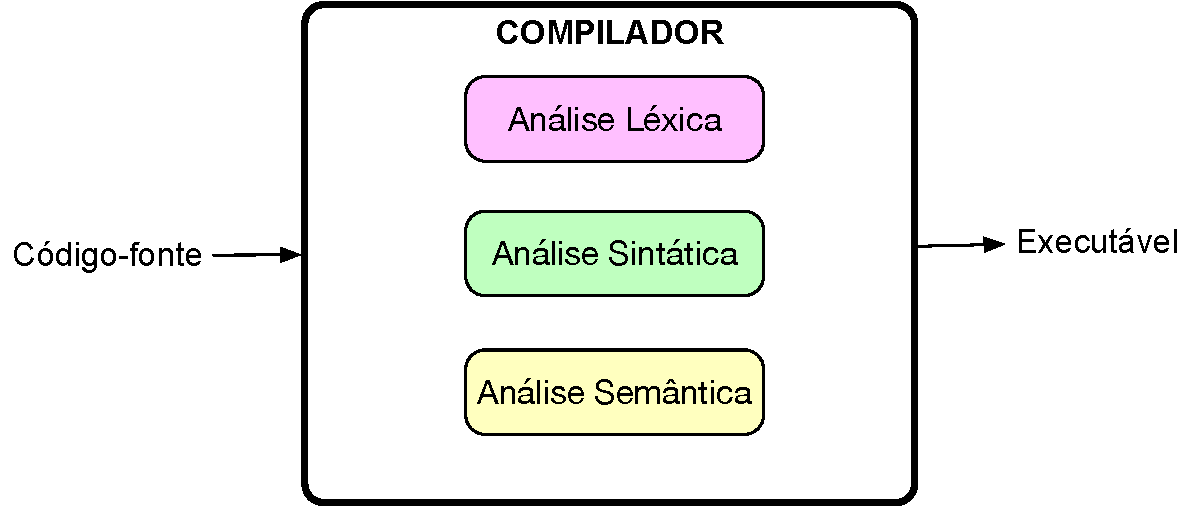
\includegraphics[scale=0.57]{figs/compilador.pdf}
\end{center}


}

\Sli{
\justifying \underline{Sintaxe:} estuda a \textbf{disposição/organização} das palavras na frase/discurso, bem como a \textbf{relação lógica} das frases entre si.\newline

\justifying Exemplos positivos:

\begin{itemize}
	\item As crianças jogam futebol.
	\item O garoto está bebendo um suco.
\end{itemize}

\justifying Exemplos negativos (sem sentido):

\begin{itemize}
	\item As crianças joga futebol (erro de \textbf{concordância}).
	\item O suco está bebendo o garoto.
	\item O garoto vai bebe a água (erro \textbf{léxico}, ou seja, de escrita).
\end{itemize}
}

\Sli{
\justifying Como seria no cotidiano de nosso curso?\newline

\justifying Exemplos positivos:
\begin{itemize}
	\item	if (x < 10) x = y;
	\item	a = 7; 
\end{itemize}

\justifying Exemplos negativos:
\begin{itemize}
	\item	if (x < 10 x = y;
	\item	7 = a; 
\end{itemize}
}

\Sli{
\justifying \underline{Semântica:} estuda o \textbf{significado} das palavras na frase/discurso. É importante para analisar o \textbf{contexto}. Erros semânticos alteram o sentido da frase.\newline

\justifying Exemplos:
\begin{itemize}
	\item Eu \emph{caminho} todos os dias.
	\item O \emph{caminho} é bastante longo até a minha escola.
	\item Fomos pegos. A \emph{batata} assou.
	\item Eu acertei todas as questões da prova. Isso é \emph{batata}!
	\item Eu gosto de \emph{batata} assada.
\end{itemize}
}

\Sli{
\justifying Como seria no cotidiano de nosso curso?\newline

\justifying Exemplo de erro semântico, ou seja, o programa \textbf{não é aceito} pela linguagem.

\begin{algorithm}
\STATE{include <stdio.h>}
\STATE{$\vdots$}
\STATE{int x;}
\STATE{$\vdots$}
\STATE{x = 1.2;}
\STATE{$\vdots$}
\end{algorithm}
}

\SliT{Conceitos Básicos}{
\justifying Algumas definições:

\begin{itemize}
	\item \underline{Linguagem:} uso da palavra articulada ou escrita como meio de expressão ou comunicação entre pessoas. Para isso, precisamos de um \textbf{alfabeto}, uma \textbf{cadeia de caracteres} e um \textbf{conjunto de regras}.
	\item \underline{Alfabeto:} dizemos que um alfabeto $\Sigma$ é um conjunto \textbf{finito} de caracteres ou símbolos.
		\begin{itemize}
			\item Exemplo de alfabetos:		
			\begin{itemize}
				\item $\Sigma=\{a,b,c\}$.
				\item $\Sigma=\emptyset$.
			\end{itemize}
			\item Não são alfabetos:	
			\begin{itemize}
				\item $\Sigma=\{a,aa,aaa,\ldots\}$.
				\item $\Sigma=\mathbb{R}$.
			\end{itemize}
		\end{itemize}
\end{itemize}
}

\Sli{
\begin{itemize}
	\item \underline{Palavra:} sequência \textbf{finita} de caracteres ou símbolos \textbf{justapostos}.
		\begin{itemize}
		\item Exemplo dado o alfabeto $\Sigma=\{a,b\}$, podemos derivar as seguintes palavras (não limitado à estas):
			\begin{itemize}
				\item $ab, bb, aa, aba$.
				\item $\epsilon$: palavra \textbf{vazia}.
			\end{itemize}
		\item Não são palavras do alfabeto $\Sigma$: $abc, c, ad$.
		\end{itemize}	
		\item Elementos de uma palavra:	
		\begin{itemize}
				\item \underline{Prefixo}: qualquer sequência de símbolos \textbf{iniciais} de uma palavra.
				\item \underline{Sufixo:} qualquer sequência de símbolos \textbf{finais} de uma palavra.
				\item \underline{Subpalavra:} qualquer sequência de símbolos \textbf{contíguos} de uma palavra.
				\item \underline{Comprimento:} número de caracteres ou símbolos de uma palavra. Exemplo: seja $w=bala$ uma palavra sobre o alfabeto $\Sigma_1=\{a,b,l,o\}$. Temos que o comprimento de $w$ é $4$, ou seja, $|w|=4$ e $|\epsilon|=0$.
					\begin{itemize}
					\item Prefixos: $\epsilon, b, ba, bal, bala$.
					\item Sufixos: $\epsilon, a, la, ala, bala$.
					\item Subpalavra: $al, ala, la, \ldots$ (note que todo sufixo e prefixo é uma subpalavra).
					\item O que seria uma palavra em linguagens de programação? Pode ser uma linha de código ou o programa inteiro.
					\end{itemize}			
		\end{itemize}
\end{itemize}
}

\Sli{
\begin{itemize}
	\item \underline{Concatenação:} é uma operação binária entre duas palavras definida pela \textbf{justaposição} entre elas. Exemplo: dado o alfabeto $\Sigma_1$ anterior e duas palavras $w_1=bala$ e $w_2=bola$ sobre ele, temos que a concatenação de $w_1$ e $w_2$, ou seja, $w_1||w_2=w_1w_2=balabola$. 
	\item Propriedades:
	\begin{itemize}
	\item \underline{Elemento neutro:} $\epsilon w=w\epsilon=w$. Exemplo: $\epsilon w_1=\epsilon bala=bala$.
	\item \underline{Associatividade:} $w_1(w_2w_3)=(w_1w_2)w_3$, sendo $w_3$ uma palavra de $\Sigma_1$.
	\item \underline{Concatenação sucessiva:} $w_1^1=w=bala, w_1^2=(bala)^2=balabala$ e $w_1^0=\epsilon$.
	\item Dado o alfabeto $\Sigma$, temos que $\Sigma^\ast$ correspondo ao conjunto de todas as palavras possíveis sobre $\Sigma$. Note que $\Sigma^\ast$ \textbf{não} é um alfabeto!
	\item Temos que $\Sigma^+=\Sigma^\ast\backslash\{\epsilon\}$.
	\end{itemize}	
	\item \underline{Linguagem:} é um subconjunto $L$ de todas as \textbf{palavras} em $\Sigma^\ast$. Exemplos:
		\begin{itemize}
		\item $\emptyset$ e $\epsilon$ são linguagens sobre qualquer alfabeto.
		\item $\Sigma^\ast$ e $\Sigma^+$ são linguagens em qualquer alfabeto.
		\item Conjunto de palíndromes sobre um alfabeto $\Sigma$.
		\end{itemize}
	\item \underline{Linguagem de programação:} conjunto de todos os programas (palavras) da linguagem.
\end{itemize}
}

\Sli{
\justifying \textbf{Gramática} é um conjunto \textbf{finito} de regras que, quando aplicadas \textbf{sucessivas} vezes, geram \textbf{palavras}. É também utilizada para definir a semântica.\newline

\justifying Uma gramática (Gramática de Chomksy ou Gramática Irrestrita) é definida como uma 4-upla \textbf{ordenada} da seguinte forma:

\begin{equation}
	G=(V,T,P,S)\nonumber,
\end{equation}
em que:\newline
$V$: conjunto de símbolos \textbf{variáveis}.\newline
$T$: conjunto de símbolos \textbf{terminais}.\newline
$P$: conjunto de \textbf{regras de produção}.\newline
$S$: conjunto de variáveis \textbf{iniciais} da gramática.
}

\Sli{
\justifying \textbf{Exemplo:} seja o alfabeto $\Sigma=\{a,b\}$ e $L=\{bala,bola\}$ uma linguagen sobre $\Sigma$. Crie uma gramática $G$ que represente esta linguagem.\newline

\justifying Temos que $G=(V,T,P,S)$ pode ser definida da seguinte forma:\newline\newline
$V=\{A,B\}$\newline
$T=\{a,b\}$\newline
$P=\{A\rightarrow bBla,B\rightarrow a|o\}$\newline
$S=\{S\}$\newline\newline\newline
\justifying As palavras são geradas por meio de \textbf{derivações}. Temos que $L(G)$ corresponde à linguagem $L$ \textbf{gerada} pela gramática $G$. Também dizemos que duas gramáticas $G_1$ e $G_2$ são \textbf{iguais} ou \textbf{equivalentes} se elas geram a \textbf{mesma} linguagem, ou seja, $L(G_1)=L(G_2)$.
}

\Sli{
\justifying Convenções:

\begin{itemize}
	\item Letras maiúsculas: símbolos variáveis.
	\item Letras minúsculas: símbolos terminais.
	\item $w$: uma palavra qualquer.
	\item $\Sigma$: um alfabeto qualquer.
	\item $G$: uma gramática qualquer.
	\item $L$: uma linguagem qualquer.
\end{itemize}
}

\SliT{Considerações finais}{

\begin{itemize}
	\item Aprendemos sobre a importância da disciplina.
	\item Etapas léxica, sintática e semântica.
	\item Definições básicas.
\end{itemize}

}

\end{document}